\documentclass[a4paper,12pt]{article}
\usepackage[utf8]{inputenc}
\usepackage{graphicx}
\usepackage{amssymb,amsmath}
\usepackage{verbatim} 
%\usepackage{url}
\usepackage{float}
\usepackage{color}
\usepackage{listings}
\usepackage{hyperref}
\usepackage{subfig}
\pagestyle{headings}
\lstset{
basicstyle=\footnotesize,       % the size of the fonts that are used for the code
frame=single,                   % adds a frame around the code
tabsize=2,                      % sets default tabsize to 2 spaces
breaklines=true,                % sets automatic line breaking
%breakatwhitespace=false,        % sets if automatic breaks should only happen at whitespace
}
\renewcommand\contentsname{Indholsfortegnelse}
\renewcommand\refname{}
\hyphenation{cel-le-bil-le-der}
\begin{document}
	\pagestyle{empty}
	\tableofcontents
	\newpage
	
	

\pagestyle{empty}
\begin{center} %\parindent=0pt
\newcommand{\HRule}{\rule{\textwidth}{1mm}}
\vspace*{2cm}\hspace{4cm}%\stretch{0.1}}
\HRule\\[1cm]\huge{\textbf{
Detektion af vesikler i celler}}\\[0.7cm]
\huge{Bachelorprojekt}\\[1cm]
\HRule\\[3cm]
\large{Claes Nøhr Ladefoged\\[0.7cm]
       Marcus Bjerg Gregersen\\[0.7cm]}
%\vspace{1cm}%*{\stretch{2.5}}
%\large Version 0.03
%\\
 \vspace{2cm}
\end{center}
\begin{flushleft}
Juni 2011\\
\vspace{0,5cm}
Under vejledning af Jon Sporring\\
Datalogisk Institut\\
Københavns Universitet
\end{flushleft}
\newpage

\begin{abstract}
I denne rapport betragter vi problemet at detektere synaptiske vesikler i nerveceller i billeder optaget ved cryo-elektron mikroskopimetoden.
%Hvordan biologer gør det nu. Lige nu i hånden. Vi ønsker at konstruere
%Støjbetonede
Vi beskriver flere essentielle teknikker indenfor billedbehandling og benytter flere af disse på cellebillederne for at diskutere deres relevans i forhold til projektet.
%Cellebillederne der er relativt meget støj i cellebillde½ne, og 
Vi præsenterer i rapporten en metode der succesfuldt detekterer vesikler i nerveceller.
\end{abstract}

\newpage
\pagestyle{plain}
\pagenumbering{roman}
\section*{Forord}
Følgende er undertegnedes bachelorprojekt udarbejdet i perioden 31. Januar 2011 til den 10. Juni 2011 ved Datalogisk Institut Københavns Universitet, under vejledning af Professor Jon Sporring.

Vores faglige forudsætninger ved påbegyndelsen af dette projekt har været de forventede af 3. års datalogistuderende på Københavns Universitet. 
Vi er således gået ind i projektet med et solidt kendskab til en bred vifte af datalogiske problemløsningsværktøjer, men uden kendskab til de metoder der benyttes indenfor billedbehandling, herunder specielt medicinsk billedbehandling.
Det fremgår derfor også af vedlagte synopsis at en af grundpillerne for projektet, har været at tilegne os viden om en mængde teknikker indenfor billedbehandling for derefter at kunne benytte og implementere disse teknikker.
I rapporten beskriver vi således flere af de basale elementer i billedbehandling, for derefter at belyse hvorledes vi har benyttet disse til at frembringe en relativt stabil detektion af synaptiske vesikler i nerveceller.

Til sidst i projektperioden har vi haft cellebilleder til rådighed af markant højere kvalitet. Vesiklerne i disse "nye" billeder er simpelthen væsentligt tydeligere, end det er tilfældet i de gamle cellebilleder.
Vores endelige metode er således blevet til med udgangspunkt i de gamle billeder, mens vi primært har udarbejdet vores evaluering ud fra de nye cellebilleder.
Vi føler at denne fremgangsmåde er rimelig da det er vores klare overbevisning at fremtidig vessikeldetektion med Cryo-EM billeder vil foregå med billeder af mindst denne "nye" kvalitet.

Det forventes at læseren har et generelt kendskab til de forskellige metoder og termer inden for signal- og billedbehandling.

Vi vil gerne takke Postdoc Anders Lindbjerg Dahl, DTU, for at stille Sparce Label Dictionaries metoden til rådighed for os.
Ligeledes vil vi gerne takke Professor Jens Randel Nyengaard, AU, for at stille cellebillederne til rådighed for os, samt at annotere ground truth i disse.
\\
\\
\\
\begin{table}[!htb]
\begin{flushleft}
\begin{tabular}{c p{2.6cm} c}
  \underline{~~~~~~~~~~~~~~~~~~~~~~~~~~~~~~~~~~~} & & \underline{~~~~~~~~~~~~~~~~~~~~~~~~~~~~~~~~~~~}\\
  Claes Nøhr Ladefoged & & Marcus Bjerg Gregersen
\end{tabular}
\end{flushleft}
\end{table}

\newpage
\tableofcontents
\newpage

\newpage
\pagenumbering{arabic} % skifter sidetal til "tal"
\thispagestyle{plain}
\section{Introduktion}
\pagestyle{headings}
En celle i nervesystemet kaldes for en neuron eller en nervecelle. Nerveceller er de vigtigste i nervesystemet, som hjernen og rygsøjlen er en del af.
Nerveceller har bl.a. til opgave at modtage og sende information ved hjælp af elektriske og kemiske signaler. I en nervecelle er der en række synaptiske vesikler, der indeholder neurotransmittere\cite{synapticvesicle}. Nerveceller kommunikerer ved hjælp af impulssignaler. Når en nervecelle skal sende et impulssignal til en anden nervecelle, sendes en synaptisk vesikel til kanten af nervecellen og udsender neurotransmittere. Nervecellerne genskaber så de synaptiske vesikler så der igen kan sendes nye signaler. I figur \ref{fig:intro_syntrans} ses to nerveceller hvor der er markeret en synaptisk vesikel i den øverste. I den menneskelige hjerne har en synaptisk vesikel en gennemsnitlig diameter på 39.5 nm med en standard afvigelse på 5.1 nm.
\begin{figure}[H]
	\centering
	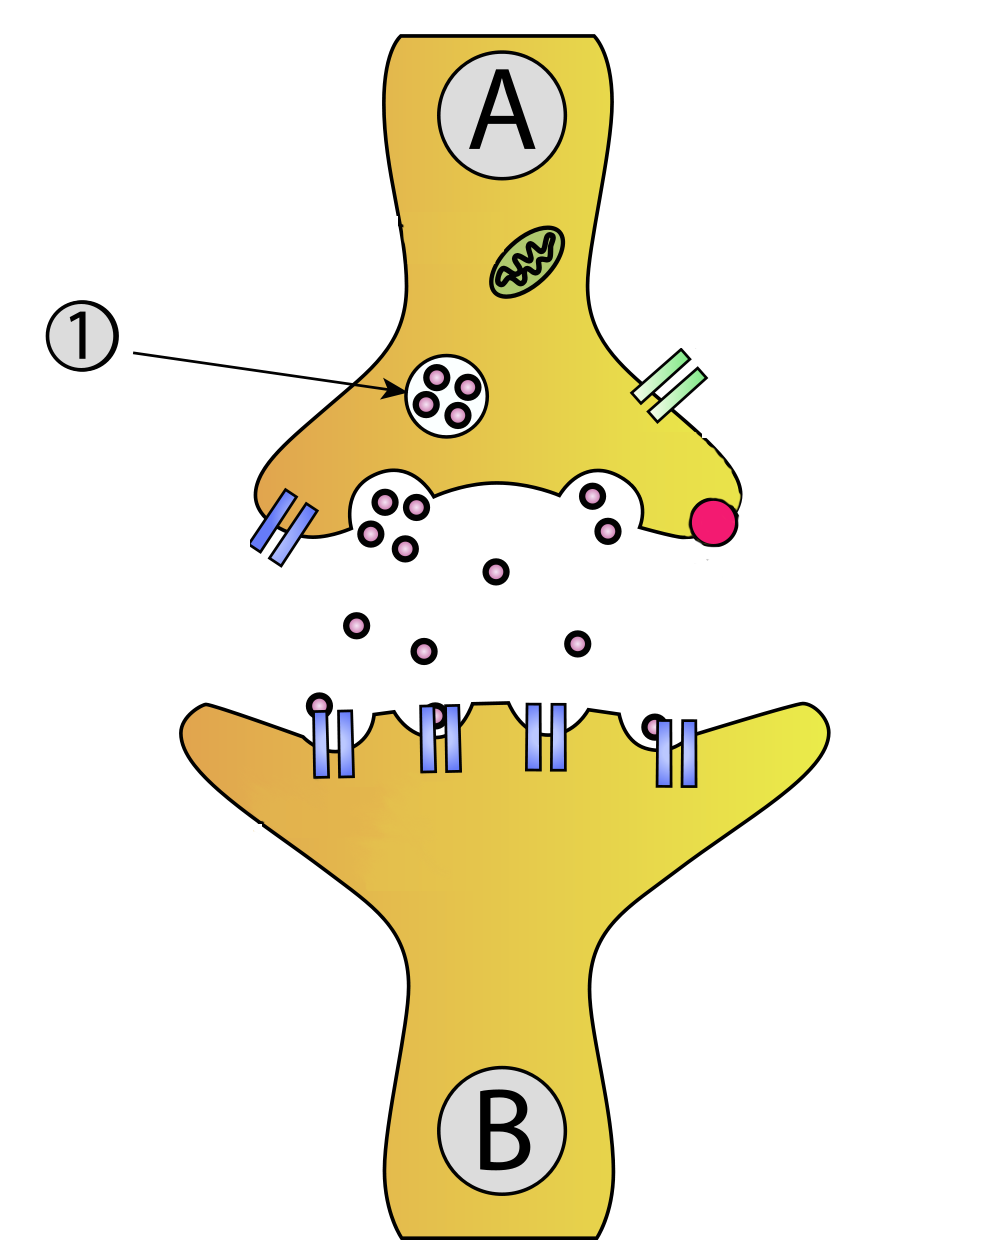
\includegraphics[scale=0.2]{files/intro/img/synTransmitter.png}
	\caption{To nerveceller, en afsender af neurotransmitters (A) og en modtager (B). Pilen peger på en synaptisk vesikel.\label{fig:intro_syntrans}\cite{neuron}}
	% Original fra : http://en.wikipedia.org/wiki/File:Synapse_diag1.svg
\end{figure} 

På Centre for Stochastic Geometry and Advanced Bioimaging (CSGA) på Aarhus Universitet, forsker Professor Jens Randel Nyengaard i mikroskopier af musehjerner. 
Forskningen går ud på at undersøge hvorvidt depression er arveligt fra mor til barn hvis moderen er deprimeret under graviditeten.
En af hypotoserne i studiet er blandt andre at man ved at observere vesiklers placering i forhold til hinanden i menneskeceller, kan sige noget om en persons sandsynlighed for at blive deprimeret. Vores problem går ud på at undersøge i hvilket omfang det kan lade sig gøre at detektere vesiklerne i cellerne.
%og lave et system der kan hjælpe forskere med at detektere disse vesikler i en celle.
Herefter vil andre efterfølgende kunne bruge denne detektion af vesikler til at analysere deres placering i forhold til hinanden, og automatisere proceduren.

Til at fremstille billederne af vesiklerne benyttes et elektronmikroskop der tager et mikroskopi af en hjerne der er frosset ned til mellem -150$^\circ$ C og -238$^\circ$ C . Disse mikroskopier er lavet ved at dele hjernen op i mange forskellige "lag" af mikroskopier.
Der vil således forekomme skygger af nerveceller fra højere eller lavere lag på et givent billede.
Da elektronmikroskopet tager billeder af mikroskopier ved meget lave temperaturer undgår man at skade cellerne unødigt, da cellerne er meget følsomme overfor stråling, der foresager meget støj i billederne. Der forekommer stadig en del støj hvilket også fremgår af billedet i figur \ref{fig:intro_celler}.
Et eksempel på en nervecelle med vesikler inden i er markeret i figuren. 
\begin{figure}[H]
	\centering
	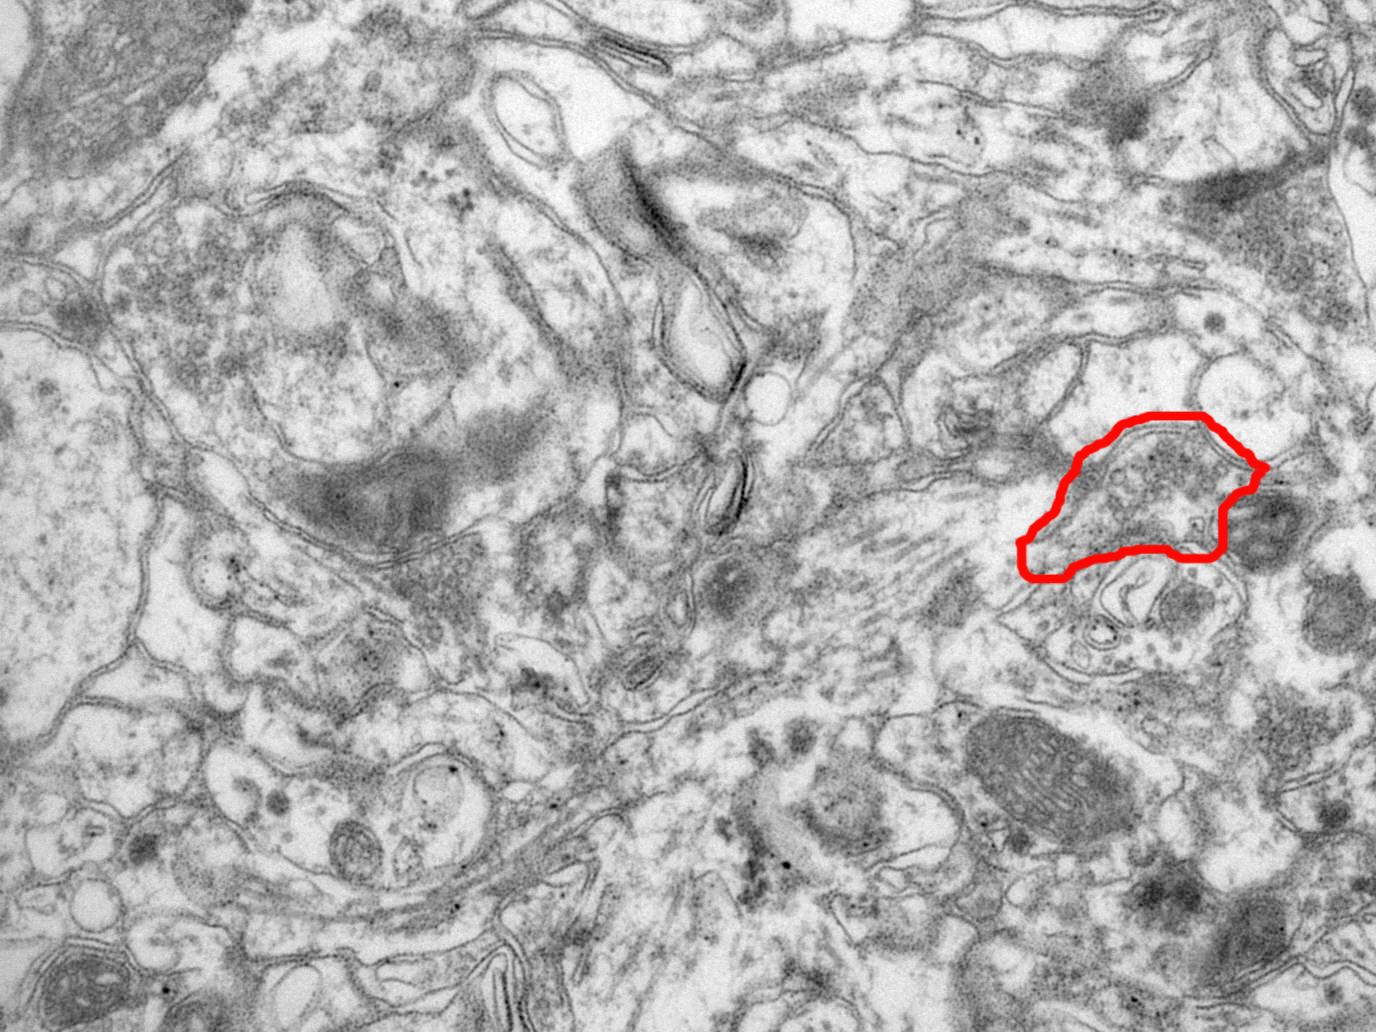
\includegraphics[scale=0.5]{files/intro/img/celler2.png}
	\caption{Billede af nerveceller taget med et elektronmikroskop. I billedet er der markeret en celle med rødt.\label{fig:intro_celler}}
\end{figure}

\subsection{Ground truth}				
Vi ønsker at detektere synaptiske vesikler i celler, og er derfor kun interesseret i billeder der indeholder en enkelt celle. Billedet til venstre i figur \ref{fig:intro_celle_groundtruth} viser et sådan udsnit. Grundet den høje støj omkring vesiklerne, er det svært at se hvor der er en vesikel, og hvor der bare er støj fra de omkringliggende vesikler eller andet som tilsammen ligner en ny vesikel. Derfor har vi i samarbejde med Professor Jens Randel Nyengaard markeret ground truth i de billeder vi behandler. Et af disse ses til højre i figur \ref{fig:intro_celle_groundtruth} hvor ground truth er markeret med lyserød prikker i hver vesikel.

\begin{figure}[H]
	\begin{minipage}[b]{0.5\linewidth}
		\centering
		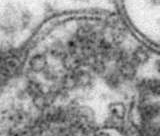
\includegraphics[scale=1.5]{files/intro/img/celle.png}
	\end{minipage}
	\hspace{0.5cm}
	\begin{minipage}[b]{0.5\linewidth}
		\centering
		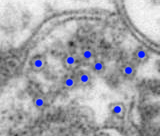
\includegraphics[scale=1.5]{files/intro/img/celle_groundtruth.png}
	\end{minipage}
	\caption{Venstre: udsnit af en enkelt nervecelle. Højre: samme udsnit med ground truth markeret med lyserøde prikker.\label{fig:intro_celle_groundtruth}}
\end{figure}

Hvis man med sine egne øjne ikke kan skelne vilkårlig støj fra en kant, vil det naturligvis også være svært at detektere alle vesikler korrekt ved hjælp af billedbehandlingsteknikker. Man kan både komme til at klassificere nogle områder der ligner en vesikel meget, men ikke er det, og omvændt kan man undlade at klassificere en vesikel, da området omkring den har så meget støj at det er svært at skælne hvor kanten stopper og støjen starter. 

\begin{figure}[H]
	\centering
	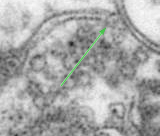
\includegraphics[scale=1.5]{files/intro/img/celle_questionves.png}
	\caption{Er der en vesikel for enden af pilen?\label{fig:intro_celle_question}}
\end{figure}

Et eksempel på et område hvor det er svært at se hvorvidt der er en vesikel ses i figur \ref{fig:intro_celle_question}. Øverst i billedet ses to områder med parallele linjer. Området mod venstre er kanten på cellen hvori vi ønsker at detektere vesikler. Den anden er kanten fra en anden celle der går lidt indover vores celle. Pilen peger så mod et område hvor de to kanter mødes, og der er meget støj. Det er svært at se med det utrænede øje hvorvidt dette er en vesikel eller bare støj. Yderligere er billederne taget ud fra meget tynde udsnit af hjernen, og det kan forekomme at man kan se skyggen af en vesikel eller celle der hører til et andet snit.  

Vores målsætning er derfor ikke at finde ground truth i alle billeder, uden at detektere en eneste falsk positiv vesikel. Succeskriteriet er blot at finde størstedelen af vesiklerne, og holde antallet af falske positiver nede.   

%% Kildehenvisninger
% http://en.wikipedia.org/w/index.php?title=Synaptic_vesicle&oldid=422206613
% http://en.wikipedia.org/w/index.php?title=Neurotransmitter&oldid=429460993
% http://en.wikipedia.org/w/index.php?title=Neuron&oldid=427379524
% http://en.wikipedia.org/w/index.php?title=Cryogenics&oldid=428358887
% http://en.wikipedia.org/w/index.php?title=Cryo-electron_microscopy&oldid=425946253



\newpage
\section{Billedbehandling}
I digital billedbehandling kan data blive repræsenteret på mange forskellige måder, alt efter hvilket domæne signalet optræder i. To af områderne er f.eks. frekvensdomænet og tid og sted domænet. Man vælger så hvilket domæne der repræsenterer de ønskede karistika i signalet bedst, ved at lave et gæt, eller ved at forsøge sig frem. Har man f.eks. observeret en række målte data, arbejder man typisk med disse i tid og sted domænet, hvor en diskret Fourier tranformation producerer information der kan aflæses i frekvensdomænet. 

Når vi ser med menneskeøjne på et billede af en celle, er de som regel uden klart defineret semantik. Da billedet bliver taget som et tværsnit kan vinklen på cellerne være lidt på kanten af en celle der gør at det er svært at se klare overgange mellem cellerne, og kanterne vil i stedet have noget støj der kan gå ud over billedet, hvilket også blev diskuteret i tidligere afsnit.

Fra et datalogisk synpunkt kan vi derfor ønske at transformere dataene i billedet til en mere kompakt repræsentation, hvor vi har lettere tilgængelighed til det semantiske indhold. Man kan forestille sig at vi er interesserede i at fjerne eller nedtone uinteressante detaljer i billedet, såsom denne støj ved cellens kant, eller fremhæve væsentlige ting, som i vores tilfælde med vessiklerne. 

En sådan reduktion af støj, eller ekstraktion af interessante konturer, opnås ved flere skridt af datamatisk analyse. Man kan f.eks se på resultatet efter en filtrering, der typisk er det første skridt i digital billedbehandling, og se efter kontraster og markant afvigende pletter i forhold til omgivelserne. Disse observationer giver så en indikation for hvilket retning den fortsatte analyse skal gå.

Da man ved filtrering ønsker flere ting, deriblandt både reduktion og ekstraktion, findes der naturligvis mange typer af filtre der kan benyttes i analysen, og det er målet for analysen der bestemmer hvilke filtre der skal benyttes. 

\subsection{Foldning og filtrering}
% Skriv om dette (kantfejl ved foldning)
%http://www.echoview.com/files/WebHelp/Reference/Algorithms/Operators/Convolution_algorithms.htm
Filtreringen foretages ofte ved en foldning af billedet med de valgte filterfunktionener. I matematik, og specielt i funktionanalyse, er foldning en matematisk operation på to funktioner, $f$ og $g$, der producerer en tredje funktion der er en modificeret funktion af en af de to funktioner. Foldning opnås ved
\begin{align}
	f(t)*g(t)=\int_{-\infty}^{\infty}f(\tau)g(t-\tau)d\tau
\end{align}
hvor $*$ er tegnet for foldning. 

Man opnår samme resultat ved at folde f og g i tid og sted domænet som man gør ved at multiplicere deres fouriertransformerede i frekvensdomænet, og så invers fouriertransformere.
\begin{align}
	f(t)*g(t) = \mathbb{F}^{-1}(\mathbb{F}(f)\cdot\mathbb{F}(g))
\end{align}
hvor $\mathbb{F}$ betyder at der er foretaget en fouriertransformation af funktionen og $\mathbb{F}^{-1}$ er en invers fouriertransformation.

Som beskrevet ovenfor er formålet ved en filtrering tit at fremhæve eller dæmpe visse frekvenser som f.eks ved at dæmpe de høje frekvenser og lade de lave passere, eller omvendt, eller at dæmpe nogle udvalgte frekvenser. 

De mest benyttede filtre er de lineære positionsinvariante.\footnote{Forelæsningsnoter til introduktion til billedbehandling, 25. oktober 2006, side 39} Et filter er lineært hvis det kan skrives som et lineært udtryk $O=\mathbf{F}I$ hvor $I$ hhv. $O$ er input hhv. output billeder organiseret som søjlevektorer og $\mathbf{F}$ er en kvadratisk matrix af filterværdier. 

Man kan filtrere billederne i både frekvendomænet og tid og sted domænet. Signaler kan konverteres fra tid og sted domænet til frekvensdomænet, og tilbage igen, gennem fouriertransformation.

\subsubsection{Lav-pas filtrering}
Ved en lav-pas filtrering dæmpes de høje frekvenser og de lave frekvenser får altså lov at passere. Lav-pas filtrering er en effektiv metode til at undertrykke støjen, men ulempen er at der sker en reduktion i kontrasten fordi højfrekvent energi fra billedkontraster ikke kan skelnes fra højfrekvent energi fra støj.

Der findes her en række af filtre såsom Ideal filtret, Butterworth filtret, Hanning filtret og Gauss filtret. Forskellen i disse filtre er hvordan de efterlader billedet. Da lav-pas filtret også dæmper de høje frekvensers energi fra billedkontraster kan man f.eks ved Ideal filtret opleve ringningseffekt omkring kraftige kontraster i billedet. Butterworth filtret har kun i meget ringe grad ringningseffekt da filtret tillader en portion af høje frekvenser at passere og derfor er "cut-off"-frekvensen glat. Det mest benyttede filter er Gauss filtret.\footnote{Forelæsningsnoter til introduktion til billedbehandling, 25. oktober 2006, side 43}

\subsubsection{Høj-pas filtrering}
Hvor lav-pas filtrering altså dæmpede de høje frekvenser og dermed kontraster og støj, har høj-pas filtrene til formål at fremhæve kontraster ved at dæmpe de lave frekvenser. 

\subsubsection{Bånd-pas filtrering}
Ved en bånd-pas filtrering tillades kun et bestemt frekvensbånd at passere. Passagen kan ske uhindret som i et ideal bånd-pas filter eller dæmpes glat ved overgangen mellem de frekvenser, der passerer, og de, der undertrykkes. Hvis der forekommer meget regelmæssig støj i et billede, vil denne støj optræde som punkter med numerisk stor værdi i styrkespektret for billedet. Det er ofte muligt at se sådanne punkter i et logaritmisk plot af styrkespektret.

\subsection{Tid og sted domænet}
Filtrering i tid og sted domænet foretages med fordel, når støtten for filtret er lille. Fordelen ved filtrering i tid og sted domænet bliver særlig stor hvis filtret er separabelt. 

% Hvad er støtten????
Hvis filtreringens formål er at fjerne støjen, og støtten for filtret er stor, vil filtrets egenskab mht. undertrykkelse af støj som regel være god. Generelt er det nødvendigt at øge støtten jo ringere signal-støjforholdet i et billede er. Signal-støjforholdet er defineret ved forholdet mellem energien i signalet og energien i støjen. Hvis filtreringens formål er at producere et billede til efterfølgende menneskelig inspektion, vil det imidlertid ofte ære en fordel at holde støtten lille.

To meget benyttede filtre er Box filtret og Gauss filtret. En egenskab ved Gauss filtret er at dette filter vil fremkomme ved gentagende filtrering af et vilkårligt filter med sig selv.\footnote{Forelæsningsnoter til introduktion til billedbehandling, 25. oktober 2006, side 46}

\subsection{Frekvensområdet}
Hvor tid og sted domænet f.eks. viser grafer over hvordan signalet ændrer sig over tid, viser grafen i frekvensområdet i stedet hvor meget af signalet der ligger inden for en række frekvenser der danner et bånd. I frekvensområdet arbejder man med fouriertranformationer.

\subsubsection{Fouriertransformation}
Fouriertransformation kommer fra studierne i Fourierserier, der i matematikens verden, er en måde at dekomposere et hvilken som helst periodisk signal til summen af et sæt af simple svingende funktioner, f.eks sinus og cosinus. Fourierserier blev introduceret af Joseph Fourier (1768-1830) med formålet at løse varmeligningen i en metalplade.

Navnet Fouriertransformation refererer både til frekvensdomænet af signalet og processen der transformerer signalet til dets frekvensdomænerepræsentation. Fouriertransformation er klassisk inden for al signal- og billedbehandling. Dette skyldes bl.a. at en række foldninger kan beregnes væsentlig hurtigere ved brug af fouriertransformationen. Fouriertransformationen giver mulighed for visuelt at fortolke billedet på en ny måde og for at specificere visse filtre lettere. Matematisk set er fouriertransformationen blot en ud af mange baseskiftende transformationer.

% SKRIV MERE MATEMATISK HVAD FOURIERTRANSFORMATION ER.

% VIS EKSEMPLER PÅ BILLEDER I FOURIER OMRÅDER OG VIS SKRIDTERE GRAFISK

%% Referencer:
% http://en.wikipedia.org/w/index.php?title=Digital_signal_processing&oldid=426007207
% http://en.wikipedia.org/w/index.php?title=Frequency_domain&oldid=424506778
% Forelæsningsnoter til introduktion til billedbehandling, 25. oktober 2006

\newpage
\thispagestyle{plain}
\section{Programmeringsprog}
\pagestyle{headings}
Da vi skulle vælge hvilket værktøj vi ville implementere vores projekt i gjorde vi os ikke specielt mange overvejelser. 
Vores valg faldt hurtigt på Python, Numpy og Scipy, da vi tidligere havde stiftet bekendskab med MATLAB, og begge var af samme opfattelse nemlig
at syntaksen i MATLABs scripingsprog langt fra var behageligt at arbejde med.


Vi har derfor bygget et framework i Python der kraftigt gør brug af Numpy. Frameworket består af 4 filer: \texttt{proc.py, functions.py, main.py, constants.py}.

I \texttt{functions.py} ligger alle vores funktioner, disse inkluderer for eksempel: foldning med en gausskerne og difference of gaussians.
\texttt{constants.py} indeholder forskellige konstanter og foldningskerner. I \texttt{proc.py} kan funktionerne kaldes med forskellige parametre, på et eller flere billeder, i den rækkefølge man ønsker.
En procedure har følgende syntaks:
\begin{verbatim}
PROCEDURE_NAVN = (BILLEDSTI, [
                 (funktion1,
                   {eventuelle parametre til funktion1}),
                 (funktion2,
                   {parametre til funktion2}),])
\end{verbatim}
I nedenstående kode giver vi et konkret eksempel på en procedure der indlæser et billede, bygger en gausskerne som beskrevet i afsnittet \nameref{sec:premethod_gaussblur}, og folder billedet med denne kerne, for til sidst at vise resultatet på skærmen:
\begin{figure}[H]
\begin{verbatim}
manuel_gauss_test = ( 
    'img/cirkel.png',
    [
    (manual_gauss,{
        'sigma':7,
        'x0':0,
        'y0':0
    }),
    (display,{})],
    )
\end{verbatim}
%\label{mis:sprog_manuel_gauss}
\end{figure}
Funktionerne bliver udført som forventet, i den rækkefølge de forekommer i listen.
Da vi i flere af de metoder vi benytter os af behøver de helt rigtige parametre for at opnå et brugbart resultat, har ovenstående syntaks vist sig at være meget nyttig da alle parametre ændres i samme fil.

Herefter tilføjes proceduren til en liste af flere andre procedurer. Denne liste pakkes ud og håndteres i \texttt{main.py}. Vores framework kaldes således: 
\begin{verbatim}
	python main.py <indeks i procedurelisten>
\end{verbatim}
Kaldet \texttt{'python main.py 0'} ville således kunne frembringe proceduren\\ \texttt{manuel\_gauss\_test}·

Vi har været glade for at have haft dette framework som 
%læringsværktøj
læringssandkasse men det har vist sig at det til vores projekt er MATLAB underlegent af flere grunde:
\begin{itemize}
	\item Numpy/Scipy er ikke specielt tolerant overfor programmeringsfejl. De stacktraces der udskrives ved fejl bringer blot information om hvilke interne Numpy-funktioner der fejler, og hjælper ikke brugeren i retningen af en mulig løsning. Dette er tilfældet i selv nogle af de simpleste tilfælde, f.eks. ved matrixmultiplikation af to matricer af inkombatible dimensioner. %i numpy 1.5.1.
	% \item Vi er flere gange i udviklingsforløbet stødt ind i at navngivningen af metoder i Scipy/Numpy er inkonsistent og ret forvirrende. 
	% \item I Numpy/Scipy findes der ofte 2 udgaver af den samme metode, forskellen på disse er blot at den ene modtager 1-dimensionelle arrays (vektorer) som input, og den anden modtager et 2-dimmensionelt array (matricer) som input. Man har således både \texttt{scipy.signal.convolve()} og \texttt{scipy.signal.convolve2d()}. Dette konkrete eksempel er også tilfældet i MATLAB, her findes dog \texttt{conv()} der er en overloadet metode der selv håndterer hvilken funktion der kaldes afhængig af input.
	\item Dokumentationen til Numpy og i særdeleshed Scipy er mangelfuld og i sjældne tilfælde ikke eksisterende. 
\end{itemize}

Både MATLAB og Python har en interaktiv shell hvor man kan udforske forskellige af de indbyggede metoder på kørselstidspunktet. Begge miljøer understøtter kaldet \texttt{help()} der fremkalder dokumentationen af en funktion på kørselstidspunktet, problemet ved scipy/numpy er som sagt blot at den vedlagte dokumentation til tider er noget sparsom.

Vi er ligeledes kommet til konklusionen at MATLAB har væsentligt flere funktioner der har været meget bekvemme i vores tilfælde. Af disse kan nævnes \texttt{nlfilter} der flytter, en af inputargumentet bestemt kvadratisk "kasse", pixel for pixel, og udfører en brugerbestemt funktion på hvert udsnit. Det er således rart at man ikke skal bekymre sig om at implementere nlfilteret men kan koncentrere sig om hvad den skal gøre. 
Vi har derfor valgt at implementere vores endelige værktøj i MATLAB, da vi har fundet at vi har kunnet producere fungerende kode hurtigere med MATLAB end med Numpy/Scipy. %\bf{MERE} 


\newpage
\section{Forsøgte metoder} %
\subsection{Metoderne}	   %
\subsubsection{Hough detektion}
\subsubsection{Edge detektion}
\subsubsection{subsubsection name}
\subsection{Reflektion}    %

\section{Endelige metode}
\subsection{Metoderne}
\subsubsection{Sparse Label Dictionaries}	% Marcus
%\textbf{Disclaimer der måske skal med: SLD er en metode udviklet af Anders noget fra DTU, vi har set metoden til et foredrag men har ikke set noget litteratur der beskriver metoden udførligt. Dette er derfor vores udlægning af SLD-metoden}\\
%\\
SLD er en metode til at klassificere forskellige elementer i et givent billede. I SLD vælger man et passende udsnit af kandidatbilledet hvorefter 


Sparse Label Dictionaries-metoden (SLD) vælger man et passende udsnit af kandidatbilledet således at udsnittet kommer til at indeholde de forskellige klasser af elementer man ønsker at dedektere samt



\subsubsection{Foldning med eksempelbilleder} % Marcus
\subsubsection{Kombinationen} % Marcus
\subsection{Evaluering}
\subsubsection{ROC}
\subsubsection{Forbedringer af endelige metode}
\subsubsection{Hvad arbejder andre med} %


\newpage
\thispagestyle{plain}
\section{Konklusion}
\pagestyle{headings}


\newpage
\thispagestyle{plain}
\section{Litteratur}
\pagestyle{headings}
\bibliographystyle{unsrt}
\bibliography{bibtexfile}

\newpage
\thispagestyle{plain}
\section{Appendix}
\subsection*{Synopsis}
\subsubsection*{Projektets titel}
Detektion af vesikler i celler.

\subsubsection*{Problemformulering for projektet}
At konstruere et program der automatisk detekterer synaptiske vesikler i celler, ud fra et billedudsnit der indeholder en enkelt celle. 
%Derefter vil vi sammenholde dette med ground truth for samme billede udpeget af biologer. 

\subsubsection*{En afgrænsning af problemformuleringen som beskriver eventuelle emner eller aspekter som gruppen har valgt ikke at behandle. }
Vi vil ikke behandle detektion af cellerne, og de billeder vi behandler vil derfor kun være af en enkelt celle. Vores succeskriterie er den af biologer definerede ground truth.

\subsubsection*{Begrundelse som fortæller hvorfor problemformuleringen er væsentlig og interessant. }
Biologer arbejder med billeder af celler og undersøger hvordan stress påvirker placeringen af vesiklerne i celler hos henholdsvis depressive og ikke depressive patienter under graviditet. Til forsøget benyttes billeder af rotters celler. 
% Ret ovenstående startformulering.

Forskningen kræver at man på billederne lokaliserer cellerne, vesiklerne i cellerne, og laver statistik over deres placering. Vores problem er at automatisere detekteringen af vesiklerne i cellerne.
\subsubsection*{En liste over de opgaver der skal løses for at gennemføre projektet med angivelse af forventet tidsforbrug for hver af dem. }
Vi har i alt 16 uger til projektet skal afleveres, hvor vi skal igennem nedenstående 4 punkter. Dette har vi så tegnet i nedenstående gantt diagram.
\begin{enumerate}
	\item Selvstudie i medicinsk billedbehandling
	\item Implementere algoritmer til detektion af vesiklerne i cellerne
	\item Evaluering af algoritmerne
	\item Rapportskrivning
\end{enumerate}
\begin{gantt}{5}{16}
    \begin{ganttitle}
      \numtitle{1}{1}{16}{1}
    \end{ganttitle}
    \ganttbar{(1)}{0}{9}
    \ganttbar{(2)}{1}{10}
    \ganttbar{(3)}{9}{5}
    \ganttbar{(4)}{0}{16}
\end{gantt}

% \begin{gantt}{4}{8}
% 	\centering
%     \begin{ganttitle}
%       \numtitle{1}{1}{8}{1}
%     \end{ganttitle}
%     \ganttbar{Rapportskrivning}{0}{8}
%     \ganttbar{Selvstudie}{0}{8}
%     \ganttbar{Algoritmeimplementering}{1}{7}
% \end{gantt}
% 
% \begin{gantt}{4}{8}
% 	\centering
%     \begin{ganttitle}
%       \numtitle{9}{1}{16}{1}
%     \end{ganttitle}
%     \ganttbar{Rapportskrivning}{0}{8}
%     \ganttbar{Algoritmeimplementering}{0}{7}
%     \ganttbar{Færdiggøre endelige program}{2}{5}
% \end{gantt}

\subsubsection*{Evt. metodiske overvejelser, relevant litteratur eller andet der kan uddybe og begrunde listen over opgaver.}
Vi vil tage udgangspunkt i bogen \emph{Bernd Jähne, "Digital Image Processing", 6. udgave} hvori vi vil benytte kapitel 1-3. Yderligere vil vi benytte Søren Olsens noter til kurset \emph{Introduktion til Billedbehandling} fra 2006-2007.

Vi vil studere forskellige metoder til at detektere vesikler og vælge de der producerer det bedste resultat. Vi vil sammenholde vore resultater med ground truth for at optimere vores algoritmer.

\subsubsection*{Læringsmål}
Vi ønsker at tilegne os viden om en mængde af teknikker indenfor billedbehandling og derefter kunne analysere og implementere disse til at løse delopgaver i vores problem. Et af vore læringsmål er derfor at kunne benytte en tillært teknik på vores datasæt og analysere resultatet og evaluere dette i forhold til andre metoder. Vi ønsker at fremvise disse forskellige metoder, samt diskutere fordele og ulemper, for derefter at præsentere vores endelige løsning på problemet.

\end{document}
